
\begin{figure}[htb] % K4 and its subdivision
  \centering
  \subfigure[Graph $G$] {
    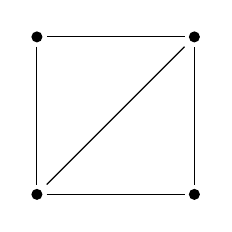
\begin{tikzpicture}
      \node (n1) at (0,0) {};
      \node (n2) at (2,0) {};
      \node (n3) at (2,2) {};
      \node (n4) at (0,2) {};
      \foreach \i in {1,...,4} {
	\fill (n\i) circle(2pt);
      };
      \foreach \i/\j in {1/2, 2/3, 3/4, 4/1, 1/3} {
	\path (n\i) edge (n\j);
      };
    \end{tikzpicture}
  }
  \subfigure[subdivision $H$ of $G$] {
    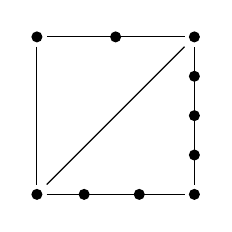
\begin{tikzpicture}
      \node (n1) at (0,0) {};
      \node (n2) at (2,0) {};
      \node (n3) at (2,2) {};
      \node (n4) at (0,2) {};
      \node (n5) at (0.6,0) {};
      \node (n6) at (1.3,0) {};
      \node (n7) at (2,.5) {};
      \node (n8) at (2,1.0) {};
      \node (n9) at (2,1.5) {};
      \node (n10) at (1,2) {};
      \foreach \i in {1,...,10} {
	\fill (n\i) circle(2pt);
      };
      \foreach \i/\j in {1/2, 2/3, 3/4, 4/1, 1/3} {
	\path (n\i) edge (n\j);
      };
    \end{tikzpicture}
  }
  \caption{Graph $G$ and one possible subdivision of $G$ named $H$}
\end{figure}


